\documentclass[border=8pt]{standalone}
\usepackage{tikz}
\usepackage{amsmath,amssymb}
\usetikzlibrary{arrows.meta,positioning,shapes.geometric,fit,calc,decorations.pathreplacing,backgrounds}

% Colors from color_schema.json
\definecolor{cprimary}{HTML}{2D5F8A}
\definecolor{cprimarylight}{HTML}{5B8DB8}
\definecolor{cprimarydark}{HTML}{1A3A5C}
\definecolor{csecondary}{HTML}{C25B28}
\definecolor{csecondarylight}{HTML}{E8925F}
\definecolor{caccent}{HTML}{3A8C6E}
\definecolor{caccentlight}{HTML}{6BB89A}
\definecolor{cwarning}{HTML}{D4A843}
\definecolor{cneutraldark}{HTML}{333333}
\definecolor{cneutralmid}{HTML}{888888}
\definecolor{cneutrallight}{HTML}{CCCCCC}
\definecolor{bgencoder}{HTML}{E8F0F8}
\definecolor{bgpredictor}{HTML}{FFF3E8}
\definecolor{bgtarget}{HTML}{E8F8F0}
\definecolor{bgloss}{HTML}{FFF8E8}
\definecolor{bgpast}{HTML}{DDEAF6}
\definecolor{bgfuture}{HTML}{DEF0E8}
\definecolor{carrow}{HTML}{555555}
\definecolor{bgprobe}{HTML}{F5EEF8}
\definecolor{cprobe}{HTML}{7B4F9D}
\definecolor{csigreg}{HTML}{8B4513}
\definecolor{bgsigreg}{HTML}{FDF0E6}

\begin{document}
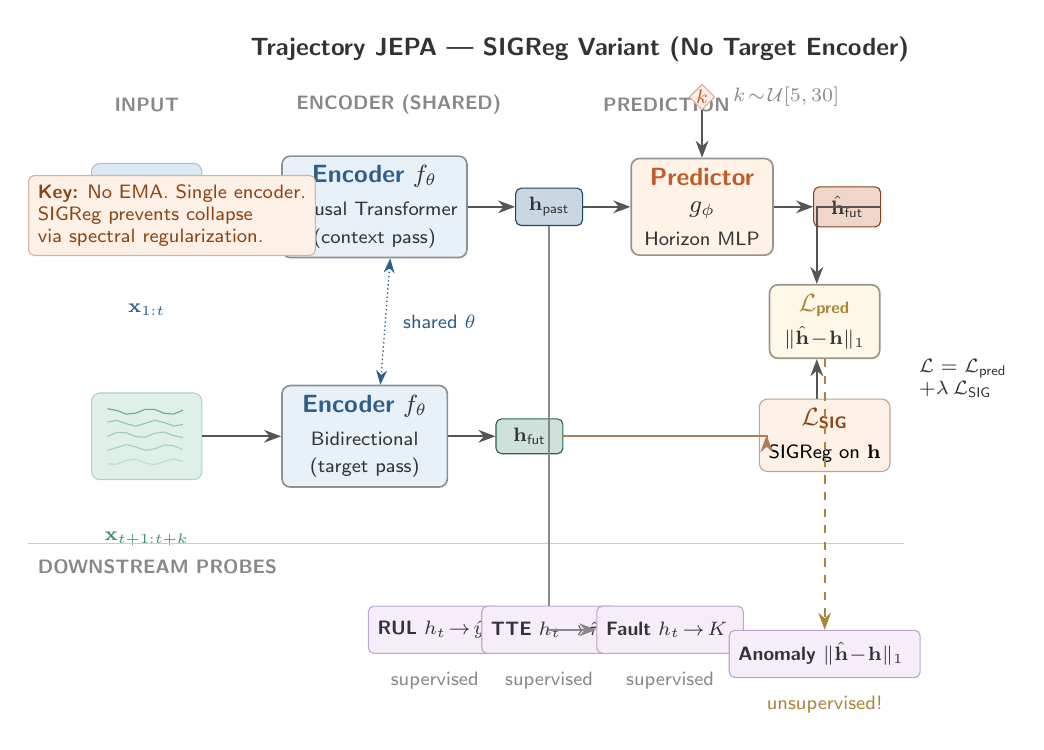
\begin{tikzpicture}[
    >=Stealth,
    font=\sffamily\small,
    block/.style={
        rounded corners=3pt,
        draw=#1!60!black,
        line width=0.6pt,
        fill=#1,
        minimum height=1.1cm,
        minimum width=2.0cm,
        align=center,
        text=cneutraldark
    },
    vec/.style={
        rounded corners=2pt,
        draw=#1!70!black,
        fill=#1!25,
        minimum height=0.32cm,
        minimum width=0.85cm,
        align=center,
        font=\sffamily\scriptsize,
        text=cneutraldark
    },
    probe/.style={
        rounded corners=2pt,
        draw=cprobe!50,
        fill=bgprobe,
        minimum height=0.6cm,
        minimum width=1.5cm,
        align=center,
        font=\sffamily\scriptsize,
        text=cneutraldark
    },
    dataarrow/.style={->,line width=0.7pt,carrow},
    section/.style={font=\sffamily\scriptsize\bfseries,text=cneutralmid},
]

% ============================================================
% TITLE
% ============================================================
\node[font=\sffamily\small\bfseries,text=cneutraldark] at (5.5,3.2)
    {Trajectory JEPA --- SIGReg Variant (No Target Encoder)};

% ============================================================
% COLUMN 1: Input time series
% ============================================================

\node[section] at (0,2.5) {INPUT};

% Past window
\node[rounded corners=3pt, draw=cprimary!40, fill=bgpast,
    minimum height=1.1cm, minimum width=1.4cm] (past) at (0,1.2) {};
\foreach \yoff/\col in {0.35/cprimary,0.18/cprimarylight,0.0/cprimary!60,
                        -0.18/cprimarylight!80,-0.35/cprimary!40} {
    \draw[thin,\col,opacity=0.7] ([xshift=-0.5cm,yshift=\yoff cm]past.center)
        \foreach \x in {0,0.12,...,0.88} { -- ++(0.12,{0.04*sin(\x*800+\yoff*200)}) };
}
\node[font=\sffamily\scriptsize,cprimary] at ([yshift=-0.75cm]past.south) {$\mathbf{x}_{1:t}$};

% Future window
\node[rounded corners=3pt, draw=caccent!40, fill=bgfuture,
    minimum height=1.1cm, minimum width=1.4cm,
    below=1.8cm of past] (future) {};
\foreach \yoff/\col in {0.35/caccent,0.18/caccentlight,0.0/caccent!60,
                        -0.18/caccentlight!80,-0.35/caccent!40} {
    \draw[thin,\col,opacity=0.7] ([xshift=-0.5cm,yshift=\yoff cm]future.center)
        \foreach \x in {0,0.12,...,0.88} { -- ++(0.12,{0.05*sin(\x*700+\yoff*300+100)}) };
}
\node[font=\sffamily\scriptsize,caccent] at ([yshift=-0.75cm]future.south) {$\mathbf{x}_{t+1:t+k}$};

% ============================================================
% COLUMN 2: SINGLE Encoder (shared weights)
% ============================================================

\node[section] at (3.2,2.5) {ENCODER (SHARED)};

% Context encoding pass
\node[block=bgencoder,minimum width=2.1cm,right=1.0cm of past] (encoder) {
    \textbf{\textcolor{cprimary}{Encoder}} $f_\theta$\\[1pt]
    {\scriptsize Causal Transformer}\\[-1pt]
    {\scriptsize (context pass)}
};
\draw[dataarrow] (past.east) -- (encoder.west);

% Future encoding pass (same encoder, different mask)
\node[block=bgencoder,minimum width=2.1cm,right=1.0cm of future] (encoder_fut) {
    \textbf{\textcolor{cprimary}{Encoder}} $f_\theta$\\[1pt]
    {\scriptsize Bidirectional}\\[-1pt]
    {\scriptsize (target pass)}
};
\draw[dataarrow] (future.east) -- (encoder_fut.west);

% Shared weights indicator
\draw[<->,line width=0.5pt,cprimary,densely dotted]
    ([xshift=0.2cm]encoder.south) -- ([xshift=0.2cm]encoder_fut.north)
    node[midway,right=0.1cm,font=\sffamily\scriptsize,cprimary] {shared $\theta$};

% ============================================================
% COLUMN 3: Representations + Predictor + SIGReg
% ============================================================

\node[section] at (6.6,2.5) {PREDICTION};

% h_past
\node[vec=cprimary,right=0.6cm of encoder.east] (hpast) {$\mathbf{h}_\text{past}$};
\draw[dataarrow] (encoder.east) -- (hpast.west);

% h_future
\node[vec=caccent,right=0.6cm of encoder_fut.east] (hfut) {$\mathbf{h}_\text{fut}$};
\draw[dataarrow] (encoder_fut.east) -- (hfut.west);

% Predictor
\node[block=bgpredictor,right=0.6cm of hpast.east,anchor=west,
    minimum width=1.8cm,minimum height=1.1cm] (predictor) {
    \textbf{\textcolor{csecondary}{Predictor}}\\[-1pt]
    $g_\phi$\\[1pt]
    {\scriptsize Horizon MLP}
};
\draw[dataarrow] (hpast.east) -- (predictor.west);

% Horizon k
\node[diamond, draw=csecondary!50, fill=csecondarylight!15,
    minimum size=0.3cm, inner sep=0pt,
    font=\sffamily\scriptsize, text=csecondary,
    above=0.6cm of predictor.north] (horizon) {$k$};
\draw[dataarrow] (horizon.south) -- (predictor.north);
\node[font=\sffamily\scriptsize,cneutralmid,right=0.1cm of horizon]
    {$k\!\sim\!\mathcal{U}[5,30]$};

% h_hat_future
\node[vec=csecondary,right=0.5cm of predictor.east] (hfuthat) {$\hat{\mathbf{h}}_\text{fut}$};
\draw[dataarrow] (predictor.east) -- (hfuthat.west);

% ============================================================
% COLUMN 4: Losses (L1 + SIGReg)
% ============================================================

% Prediction loss
\node[block=bgloss, minimum width=1.4cm, minimum height=0.8cm]
    (loss) at ([xshift=1.3cm]$(hfuthat.east)!0.5!(hfut.east)$) {
    \textbf{\textcolor{cwarning!80!black}{$\mathcal{L}_\text{pred}$}}\\[1pt]
    {\scriptsize $\|\hat{\mathbf{h}} \!-\! \mathbf{h}\|_1$}
};
\draw[dataarrow] (hfuthat.east) -| ([xshift=-0.1cm]loss.north);
\draw[dataarrow] (hfut.east) -| ([xshift=-0.1cm]loss.south);

% SIGReg regularizer (below loss)
\node[rounded corners=3pt, draw=csigreg!50, fill=bgsigreg,
    minimum width=1.4cm, minimum height=0.8cm,
    below=0.5cm of loss, align=center] (sigreg) {
    \textbf{\textcolor{csigreg}{$\mathcal{L}_\text{SIG}$}}\\[1pt]
    {\scriptsize SIGReg on $\mathbf{h}$}
};
\draw[dataarrow,csigreg!70] (hfut.east) -| ([xshift=0.1cm]sigreg.west);

% Total loss
\node[font=\sffamily\scriptsize,cneutraldark,
    right=0.3cm of $(loss.east)!0.5!(sigreg.east)$,align=left] {
    $\mathcal{L} = \mathcal{L}_\text{pred}$\\
    $+ \lambda\,\mathcal{L}_\text{SIG}$
};

% ============================================================
% DOWNSTREAM PROBES (same as EMA version)
% ============================================================

\coordinate (bottom) at ([yshift=-0.8cm]future.south);

\draw[cneutrallight,line width=0.3pt]
    ([xshift=-0.8cm]bottom -| past.west) -- ([xshift=0.3cm]bottom -| loss.east);

\node[section,anchor=west] at ([xshift=-0.8cm,yshift=-0.3cm]bottom -| past.west)
    {DOWNSTREAM PROBES};

\coordinate (probestart) at ([yshift=-1.1cm]bottom -| hpast);
\draw[dataarrow,cneutralmid] (hpast.south) -- (probestart);

\node[probe,anchor=east] (rul) at ([xshift=-0.6cm]probestart) {
    \textbf{RUL} {\scriptsize$h_t\!\to\!\hat{y}$}
};
\draw[dataarrow,cneutralmid] (probestart) -- (rul.east);
\node[font=\sffamily\scriptsize,cneutralmid,below=0.1cm of rul] {supervised};

\node[probe,anchor=center] (tte) at (probestart) {
    \textbf{TTE} {\scriptsize$h_t\!\to\!\hat{\tau}$}
};
\node[font=\sffamily\scriptsize,cneutralmid,below=0.1cm of tte] {supervised};

\node[probe,anchor=west] (fault) at ([xshift=0.6cm]probestart) {
    \textbf{Fault} {\scriptsize$h_t\!\to\!K$}
};
\draw[dataarrow,cneutralmid] (probestart) -- (fault.west);
\node[font=\sffamily\scriptsize,cneutralmid,below=0.1cm of fault] {supervised};

\node[probe,anchor=north] (anomaly) at ([yshift=-1.1cm]bottom -| loss) {
    \textbf{Anomaly} {\scriptsize$\|\hat{\mathbf{h}}\!-\!\mathbf{h}\|_1$}
};
\draw[dataarrow,cwarning!80!black,dashed] (loss.south) -- ++(0,-0.45) -| (anomaly.north);
\node[font=\sffamily\scriptsize,cwarning!80!black,below=0.1cm of anomaly] {unsupervised!};

% ============================================================
% KEY DIFFERENCE annotation
% ============================================================
\node[rounded corners=2pt, draw=csigreg!40, fill=bgsigreg,
    font=\sffamily\scriptsize, text=csigreg, align=left,
    anchor=north west] at ([xshift=-0.8cm,yshift=-0.25cm]past.west |- encoder.north) {
    \textbf{Key:} No EMA. Single encoder.\\
    SIGReg prevents collapse\\
    via spectral regularization.
};

\end{tikzpicture}
\end{document}
